
\begin{abstract}

This paper documents the creation of the art project 'Moody Plant', an interactive plant that reacts with affectionate sounds to human proximity and touch. Depending on how it is treated, it reacts in three different moods - happy, needy, angry.  The Arduino picks up whether the plant was pet. Via a Pure Data patch, (available on Michael Reiter's  Github\cite{github} the acoustic reactions are determined.
It was created in the course 'Sonic Interaction' by Michael Reiter, Elisabeth Hacker and Hanna Br\"uhwiler and supervised by Katharina Gro\ss-Vogt. 






\end{abstract}



\begin{figure}[H]
\begin{center}
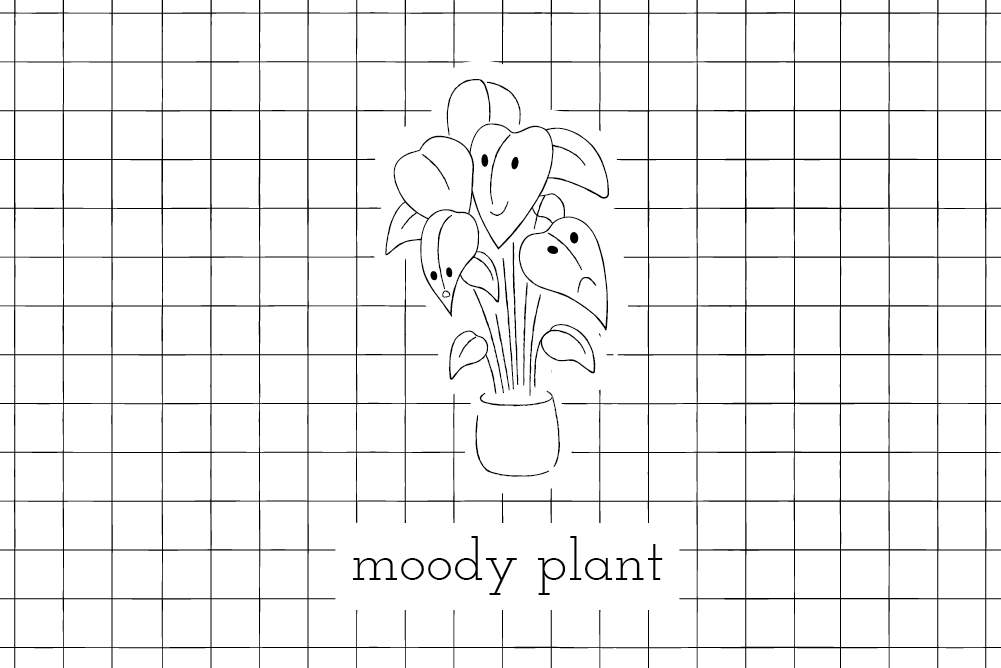
\includegraphics[scale=0.35]{Figures/thumbnail.png}
\end{center}
\end{figure}



\renewcommand{\abstractname}{Kurzfassung}
\begin{abstract}

%Eine Pflanze hat Gef\"uhle. Sie lebt wie jedes andere Lebewesen vor sich hin und wie jeder von uns, braucht sie manchmal etwas N\"ahe und Zuneigung - aber vorsicht, auch nicht zu viel! 'Moody Plant' ist eine interaktive Pflanze, welche im Rahmen eines Gruppenprojekts in Sonic Interaction Design von Michael Reiter, Elisabeth Hacker und Hanna Br\"uhwiler designt und entwickelt wurde. Ihre drei Stimmungen - fr\"ohlich, bed\"urftig, w\"utend - werden \"uber eine Arduino-Verbindung in Pure Data h\"orbar gemacht. Den PD Patch findet man auf Michael Reiters \href{https://github.com/MichaelReiter94/moody_plant}{Github}. 


Diese Arbeit beinhaltet den Entwicklungsprozess des Kunstprojektes 'Moody Plant', eine interaktive Pflanze, die auf menschliche N\"ahe und Ber\"uhrungen reagiert. Sie antwortet akustisch in drei verschiedenen Stimmungen - gl\"ucklich, bed\"urftig und w\"utend. Eine Messvorrichtung mittels Arduino erkennt, wenn die Pflanze gestrei- chelt wird und schickt diese Daten \"uber eine USB-Verbindung an einen Pure Data Patch. In diesem wird je nachdem wie die 'Moody Plant' behandelt wurde, entschieden mit welchen Kl\"angen sie reagieren soll. Der Quellcode dieses Projekts kann auf Michael Reiters Github Seite \cite{github} gefunden werden. 'Moody Plant' wurde im Rahmen des Kurses Sonic Interaction Design von Michael Reiter, Elisabeth Hacker und Hanna Br\"uhwiler entwickelt und wurde hierbei betreut von Katharina Gro\ss-Vogt. 



\end{abstract}
